%%%%%%%%%%%%%%%%%%%%%%%%%%%%%%%%%%%%%%%%%
% Engineering Calculation Paper
% LaTeX Template
% Version 1.0 (20/1/13)
%
% This template has been downloaded from:
% http://www.LaTeXTemplates.com
%
% Original author:
% Dmitry Volynkin (dim_voly@yahoo.com.au)
%
% License:
% CC BY-NC-SA 3.0 (http://creativecommons.org/licenses/by-nc-sa/3.0/)
%
% Modificaciones por Roberto Cerdas
%
% Si desea utilizar notas al margen, favor leer los comentarios en las líneas 32 y % 52. Si desea colocar un logo, favor leer comentario en línea 54. El comando     % \marginnote{texto} introduce notas al margen.  
%
%%%%%%%%%%%%%%%%%%%%%%%%%%%%%%%%%%%%%%%%%

%----------------------------------------------------------------------------------------
%	PACKAGES AND OTHER DOCUMENT CONFIGURATIONS
%----------------------------------------------------------------------------------------

\documentclass[12pt,a4paper]{article} % Use A4 paper with a 12pt font size - different paper sizes will require manual recalculation of page margins and border positions

\usepackage[spanish]{babel} % Utilizar reglas de idioma español
\usepackage[utf8]{inputenc} % Use UTF-8 encoding
\usepackage{marginnote} % Required for margin notes
\usepackage{wallpaper} % Required to set each page to have a background
\usepackage{lastpage} % Required to print the total number of pages
%\usepackage[left=1.3cm,right=4.6cm,top=1.8cm,bottom=4.0cm,marginparwidth=3.4cm]{geometry} % Comentar la línea abajo y descomentar esta para usar notas al margen
\usepackage[left=1.3cm,right=1.3cm,top=1.8cm,bottom=4.0cm]{geometry} % Adjust page margins
\usepackage{amsmath} % Required for equation customization
\usepackage{amssymb} % Required to include mathematical symbols
\usepackage{xcolor} % Required to specify colors by name
\usepackage[square, comma, sort&compress]{natbib} % Use the natbib reference package - read up on this to edit the reference style; if you want text (e.g. Smith et al., 2012) for the in-text references (instead of numbers), remove 'numbers' 

\usepackage{fancyhdr} % Required to customize headers
\setlength{\headheight}{80pt} % Increase the size of the header to accommodate meta-information
\pagestyle{fancy}\fancyhf{} % Use the custom header specified below
\renewcommand{\headrulewidth}{0pt} % Remove the default horizontal rule under the header

\setlength{\parindent}{0cm} % Remove paragraph indentation
\newcommand{\tab}{\hspace*{2em}} % Defines a new command for some horizontal space

\newcommand\BackgroundStructure{ % Command to specify the background of each page
\setlength{\unitlength}{1mm} % Set the unit length to millimeters

\setlength\fboxsep{0mm} % Adjusts the distance between the frameboxes and the borderlines
\setlength\fboxrule{0.5mm} % Increase the thickness of the border line
\put(10, 10){\fcolorbox{black}{white!10}{\framebox(192,247){}}} % Main content box
%\put(165, 10){\fcolorbox{black}{blue!10}{\framebox(37,247){}}} % Margin box: Descomentar para utilizar notas al margen.
\put(10, 262){\fcolorbox{black}{white!10}{\framebox(192, 25){}}} % Header box
%\put(143, 263){\includegraphics[height=23mm,keepaspectratio]{logo}} % Logo box - maximum height/width: 25x42. Descomentar esta línea para usar logo.
}

%----------------------------------------------------------------------------------------
%	HEADER INFORMATION
%----------------------------------------------------------------------------------------

\fancyhead[L]{\begin{tabular}{l r | l r} % The header is a table with 4 columns
\textbf{Proyecto} & Diseño inversor CMOS & \textbf{Página} & \thepage/\pageref{LastPage} \\ % Project name and page count
\textbf{Trabajo} & Análisis estático y dinámico & \textbf{Actualizado en:} & 18/09/2015 \\ % Job number and last updated date
\textbf{Versión} & 1 & \textbf{Revisado en:} & 18/09/2015 \\ % Version and reviewed date
\textbf{Diseñador} & López F. - Quirós.J.& \textbf{Revisado por:} & Alfonso Chacón Rodríguez \\ % Designer and reviewer
\end{tabular}}

%----------------------------------------------------------------------------------------

\begin{document}

\AddToShipoutPicture{\BackgroundStructure} % Set the background of each page to that specified above in the header information section

%----------------------------------------------------------------------------------------
%	DOCUMENT CONTENT
%----------------------------------------------------------------------------------------

\section{Resumen} 

En este documento se encontrará lo que es el proceso de diseño de un inversor CMOS de tamaño mínimo en la tecnología ON-semiconductor 0.5, en el cual se dimensionará el PMOS de acuerdo a un análisis estático(misma corriente en los transistores con tensión de inversion igual a la mitad de la alimentación) y a un análisis dinámico (menor tiempo de retardo en los tiempos de levantamiento y caída). También se harán los cálculos para encontrar la resistencia equivalente de los transistores NMOS y PMOS para la misma tecnología.

\section{Introducción} 

Para el diseño del PMOS del inversor, se considera el diseño del NMOS segun los parametros minimos del ancho y largo de canal (4$\lambda$/2$\lambda$) en una tecnología ON-semiconductor 0.5. Para encontrar la relación que debe tener el ancho de canal PMOS con respecto al NMOS, se tomarán en cuenta dos diferentes tipos de análisis:\\*
\\*El análisis estático el cual se busca que la corriente de NMOS y el PMOS sea simétrica. Esto se observa en que la tensión de umbral del inversor sea la mitad de la tensión de alimentación del mismo.\\*
\\*Para este análisis se plantean usar las ecuaciones de Shockley para la corriente de un transistor CMOS. Esto con el fin de graficar el comportamiento ideal de un transmisor y encontrar la relación de ancho de canal entre los transitores PMOS y NMOS.

\begin{equation}\label{eqn:NMOS_corte}
I_{dsn}=0
\end{equation}

\begin{equation}\label{eqn:NMOS_lineal}
I_{dsn}=\beta_{n}*(w_{n}/l_{n})*((2*V_{GTn})-V_{dsn})*V_{dsn}
\end{equation}

\begin{equation}\label{eqn:NMOS_sat}
I_{dsn}=\beta_{n}*(w_{n}/l_{n})*(V_{GTn})^2
\end{equation}

El análisis dinámico, se dimensionará el ancho de canal del PMOS de tal forma que el tiempo que le toma al inversor pasar de un estado lógico a otro sea el menor posible, siempre y cuando el tiempo que toma de subida y bajada de nivel lógico sean simétricos.


\section{Resultados experimentales}


\subsection{Dimensionamiento de Transistor PMOS}

\subsubsection{Análisis estático}


\begin{figure}[htbp]
  \centering
%    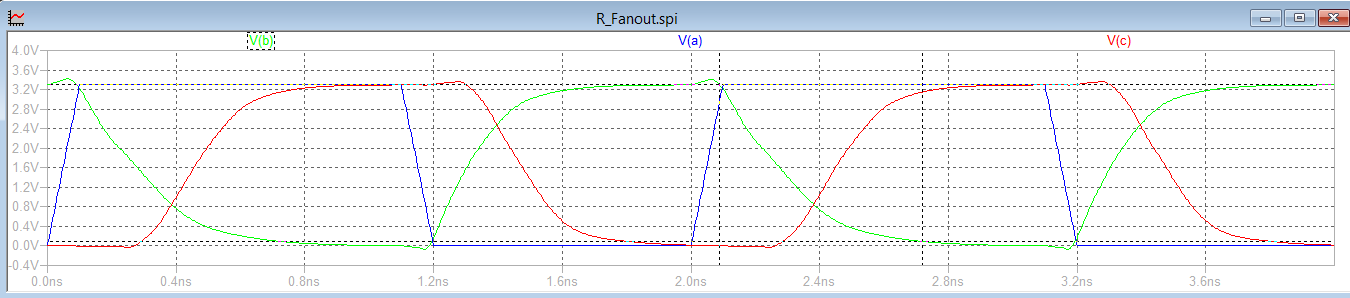
\includegraphics[scale=0.2]{./Captura.png}
    \rule{35em}{0.5pt}
  \caption[Captura]{Graficas octate ideal vs simulacion electric}
  \label{fig:inv_est}
\end{figure}

Para este análisis, primero se realizó una simulación en la plataforma de programación para cálculos matemáticos Octave, esto con el fin de tener una aproximación de la relación que debe tener el ancho de canal del PMOS con el NMOS para que la tensión de umbral del inversor $V_{inv}=V_{dd}/2$. Se utilizaron las ecuaciones en región de corte (Ec.[\ref{eqn:NMOS_corte}]), lineal (Ec.[\ref{eqn:NMOS_lineal}]) y saturación (Ec.[\ref{eqn:NMOS_sat}] y conociendo que para ciertos rangos de valores de tensión de entrada, los transistores se encontraban en regiones de polarización específicas y la tensión de salida tenia un comportamiento particular como se muestra en la tabla \ref{table:Tabla_polarizacion}.\\*
\\*

\begin{table}\label{table:Tabla_polarizacion}
\begin{center}
\begin{tabular}{c||c||c||c}
Numero & Rango entrada & Región PMOS & Región NMOS\\
\hline
\hline
1 & $V_{in}<V_{tn}$ & Lineal & Corte \\
2 & $V_{tn}<=V_{in}<V_{inv}$ & Lineal & Saturación \\
3 & $V_{in}=V_{inv}$ & Saturación & Saturación\\
4 & $V_{inv}<V_{in}<=V_{dd}+V_{tp}$ & Saturación & Lineal\\
5 & $V_{in}>V_{dd}+V_{tp}$ & Corte & Lineal\\
\hline
\end{tabular}
\caption{Regiones inversor CMOS Vin vs Vout}
\end{center}
\end{table}

Se logró la grafica [] la cual se logró encontrar que r=4 lo cual significa que el transistor PMOS debe de 4 veces más ancho que el NMOS para que las regiones sean simétricas.\\*
\\*
Para la simulación experimental, se usó el programa Electric. En esta simulación se utilizó el archivo [] para las constantes de la tecnología MOSIS 0.5, ya realizada la simulación del inversor (fig. []) con la relación de ancho de canal calculado anteriormente encontramos que la proporción de regiones en el inversor no es la esperada, por lo que se decidió volver a dimensionar el ancho de los canales con respecto a las simulaciones y encontramos que de manera experimental r=[]; 


\subsubsection{Análisis dinámico}



\subsection{Resistencia equivalente}

\subsubsection{Carga y descarga de un capacitor}


\subsubsection{Método de Fanout}

El método de Fanout plantea encontrar la resistencia equivalente de un transistor CMOS con los valores de la capacitancia parásita en el gate y el diferencial de tiempos de caída y levantamiento que le toma al mismo pasar de un nivel lógico a otro, con 2 valores de fanout distintos. Las ecuaciones para calcular las resistencias equivalentes para PMOS y NMOS son las \ref{eqn:Req_p} y \ref{eqn:Req_n} respectivamente.\\*
\\*
\begin{equation}\label{eqn:Req_p}
R_{eqp}=(2/3)*( \Delta t_{r}/C_{g})
\end{equation}

\begin{equation}\label{eqn:Req_n}
R_{eqn}= \Delta t_{f}/(3*C_{g})
\end{equation}

Se realizó la simulación del circuito propuesto encontrado en la referencia [], para valores de h=2 (fig. \ref{fig:CircuitoFO2}) y h=3 (fig. \ref{fig:CircuitoFO3} con los cuales se encontraron las graficas de los retardos de la salida con respecto a la entrada (fig. \ref{fig:FO2} y fig. \ref{fig:FO3})\\*
\\*
\begin{figure}[htbp]
\begin{center}
    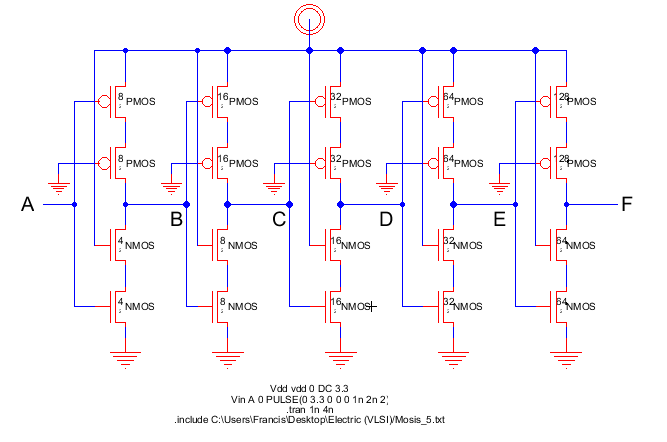
\includegraphics[scale=0.5]{./CircuitoFO2.png}
    \rule{35em}{0.5pt}
  \caption[Captura]{Circuito para calculo de $R_{eq}$ con h=2}
  \label{fig:CircuitoFO2}
  \end{center}
\end{figure}

\begin{figure}[htbp]
  \centering
    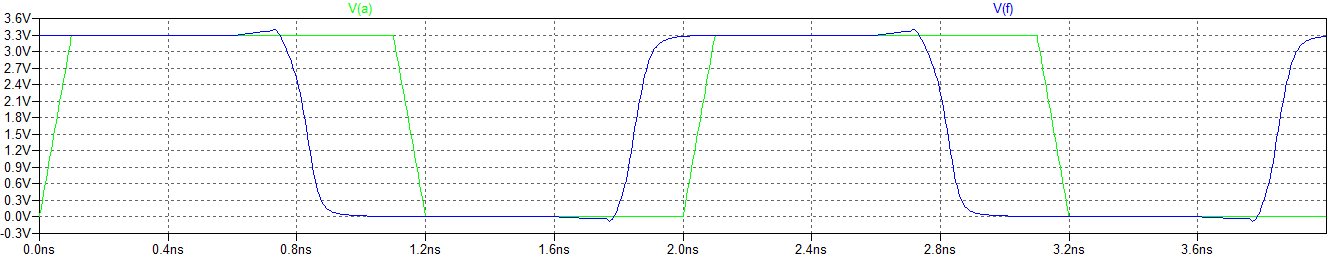
\includegraphics[scale=0.4]{./FO2.png}
    \rule{35em}{1pt}
  \caption[Captura]{Gráfica tiempo $V_{in}$ vs $V_{out}$ h=2}
  \label{fig:FO2}
\end{figure}

\begin{figure}[htbp]
\begin{center}
    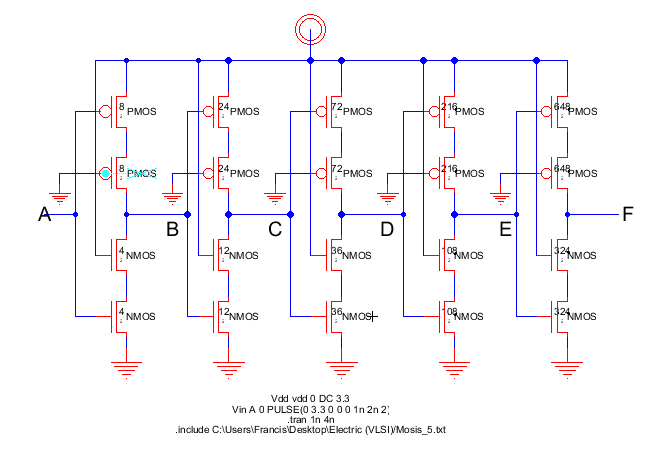
\includegraphics[scale=0.5]{./CircuitoFO3.png}
    \rule{35em}{0.5pt}
  \caption[Captura]{Circuito para calculo de $R_{eq}$ con h=3}
  \label{fig:CircuitoFO3}
  
\end{center}
\end{figure}

\begin{figure}[htbp]
  \begin{center}
    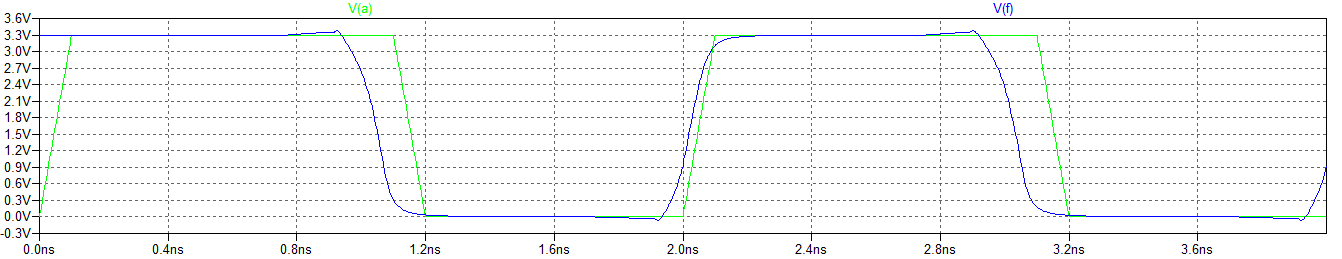
\includegraphics[scale=0.4]{./FO3.png}
    \rule{35em}{0.5pt}
  \caption[Captura]{Gráfica tiempo $V_{in}$ vs $V_{out}$ h=3}
  \label{fig:FO3}
  \end{center}
\end{figure}

Luego de encontrar las gráficas (fig. \ref{fig:FO2} y fig. \ref{fig:FO3}), se realizó la medición de los tiempos ya mencionados anteriormente. Aunque en la referencia [] se habla que la medición debe hacerse entre los valores de $0.8V_{dd}$ a $0.2V_{dd}$, se encontró que las pendientes de ambas graficas son aproximadamente iguales y no se encontraría la variación de la resistencia equivalente entre los CMOS por lo que se decidió medir de $0.9V_{dd}$ a $0.1V_{dd}$. Se encontraron los valores mencionados en el cuadro \ref{table:tiempos}. \\*
\\*
\begin{table}\label{table:tiempos}
\begin{center}
\begin{tabular}{c||c||c}
n & tr(ps) & tf(ps)\\
\hline
\hline
2 & 97.36 & 101.29 \\
3 & 117.84 & 125.055 \\
$\Delta$ & 20.44 & 23.76\\
\hline
\end{tabular}
\caption{Tiempos de levantamiento y caida de tensión para un inversor CMOS para diferentes Fanouts}
\end{center}
\end{table}


Ya con los diferenciales de tiempos medidos, se sustituyen en \ref{eqn:Req_p} y \ref{eqn:Req_n} para encontrar la resistencia equivalente de cada transistor. Para $C_{g}=1.48 fF/\mu m$  dependiente del ancho de canal de gate, se encuentra que los valores de resistencia son los del cuadro (\ref{table:resistencias}). \\*
\\*
\begin{table}\label{table:resistencias}
\begin{center}
\begin{tabular}{c||c}
Resistencia & k$\Omega$\\
\hline
\hline
$R_{eqp}$ & 15.375 \\
$R_{eqn}$ & 9.000 \\
\hline
\end{tabular}
\caption{Resistencias equivalentes encontradas por Método de Fanout}
\end{center}
\end{table}

\section{Análisis de datos y resultados}

Este proyecto ha sido un exito en el funcionamiento del controlador digital y en los circuitos acondicionaores de señal gracias a las herramientas proporcionadas, conocimientos adquiridos y metodología de trabajo que se realizaron en este laboratorio.

Los procesos de simulación tanto para los CAS como para el regulador IPD permitieron disminuir los errores que se podrian haber presentado de no haberse hecho. Para los CAS se realizaron ajustes por los valores de tolerancia de los componentes con respecto a la teoría en especial en los filtros ya que se debió ajustar las ganancias por los filtros.






\section{Conclusiones y recomendaciones}

Aquí van las conclusiones y recomendaciones del Lab.

%----------------------------------------------------------------------------------------
\begin{thebibliography}{3}

\bibliographystyle{unsrtnat} % Use the "unsrtnat" BibTeX style for formatting the Bibliography

\bibitem[Wey(1999)]{Wey1999}
C.-L.Wey and C.-P.Wang
\newblock {Design of a fast radix-4 SRT divider and its VLSI implementation}.
\newblock \emph{IEEE Proc.-Comput. Digit. Tech., IEEE}, July 1999.
\newblock DOI: 10.1049/ip-cdt:19990524.

\end{thebibliography}

\end{document}